%-----------------------------------------------------------------------------%
\chapter{ANALISIS DAN PERANCANGAN SISTEM}
%-----------------------------------------------------------------------------%
\vspace{4.5pt}
\section{Kerangka Pemikiran}
\begin{center}
	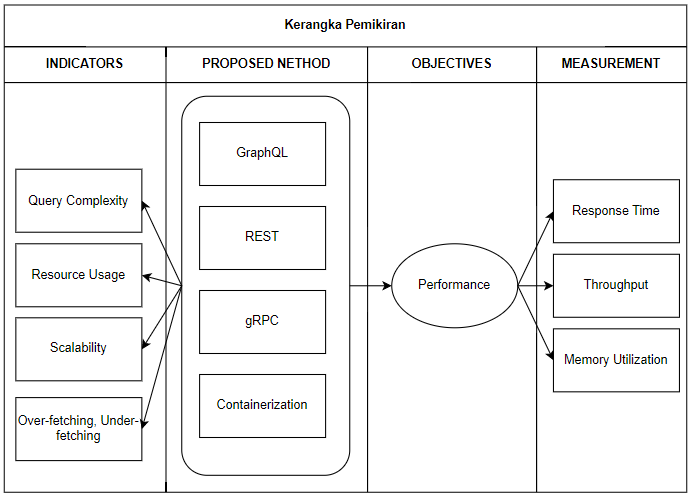
\includegraphics[width=10cm]{img/kerangka pemikiran.png}
	\captionof{figure}{kerangka pemikiran}
	\label{fig:asd}
\end{center}
Sesuai dengan rumusan masalah, pada penelitian ini terdapat satu objektif yaitu membandingkan performa  dari teknologi \textit{REST}, \textit{GraphQL} dan \textit{gRPC} yang berjalan di kotainer dan tanpa kontainer. Sebagai indikator, terdapat diantaranya \textit{query complexity}, \textit{memory usage}, jumlah pengguna \textit{(scalability)}, serta \textit{over-fetching} dan \textit{under-fetching}. Pengukuran dilakukan dengan merata-ratakan \textit{response time}, \textit{throughput}, dan \textit{memory utilization}   yang didapat dari beberapa pengujian yang diberikan.\\


\section{Urutan Proses Global}
\begin{center}
	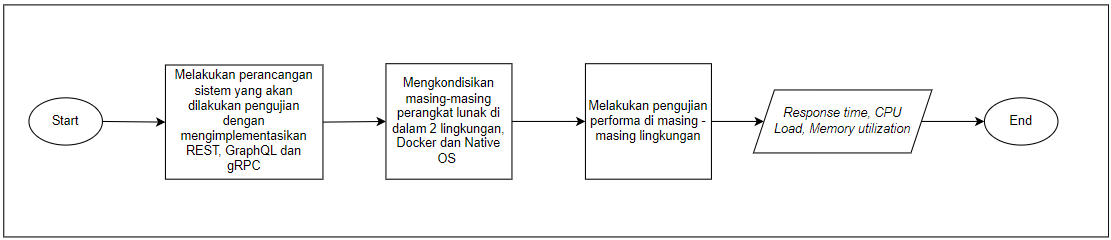
\includegraphics[width=15cm]{img/proses global.png}
	\captionof{figure}{Urutan Proses Global}
	\label{fig:asd}
\end{center}